\subsection*{Dynamical model}
We modeled the dynamics of two pathogen strains under variable amounts of competition and process noise (Fig.~\ref{fig:compartmental}).
The state variables in the system are the hosts' statuses with respect to each strain \cite{Gog2002}. 
Hosts can be susceptible ($S_i$), infected ($I_i$), or recovered and immune ($R_i$) to each strain $i$. 
The deterministic model has the form:

\begin{align}
\frac{dS_i}{dt} &=
    \mu
    - S_i\sum\limits_{j}
    \sigma_{ij}
    \beta_j(t) 
    I_j
    - \mu S_i \\
\frac{dI_i}{dt} &= 
    \beta_i(t) S_i I_i
    - (\nu_i + \mu) I_i \\
\frac{dR_i}{dt} &=
    \nu_i I_i
    + S_i\sum\limits_{j \neq i} \sigma_{ij} \beta_j(t)  I_j
    - \mu R_i \\
\beta_i(t) &= \beta_i
    \left(
        1 + \varepsilon \sin \left[
            \frac{2\pi}{\psi} \left( t - \psi \right)
        \right]
    \right) \\
S_i + I_i + R_i &= 1
\end{align}

\begin{figure}
    \begin{center}
        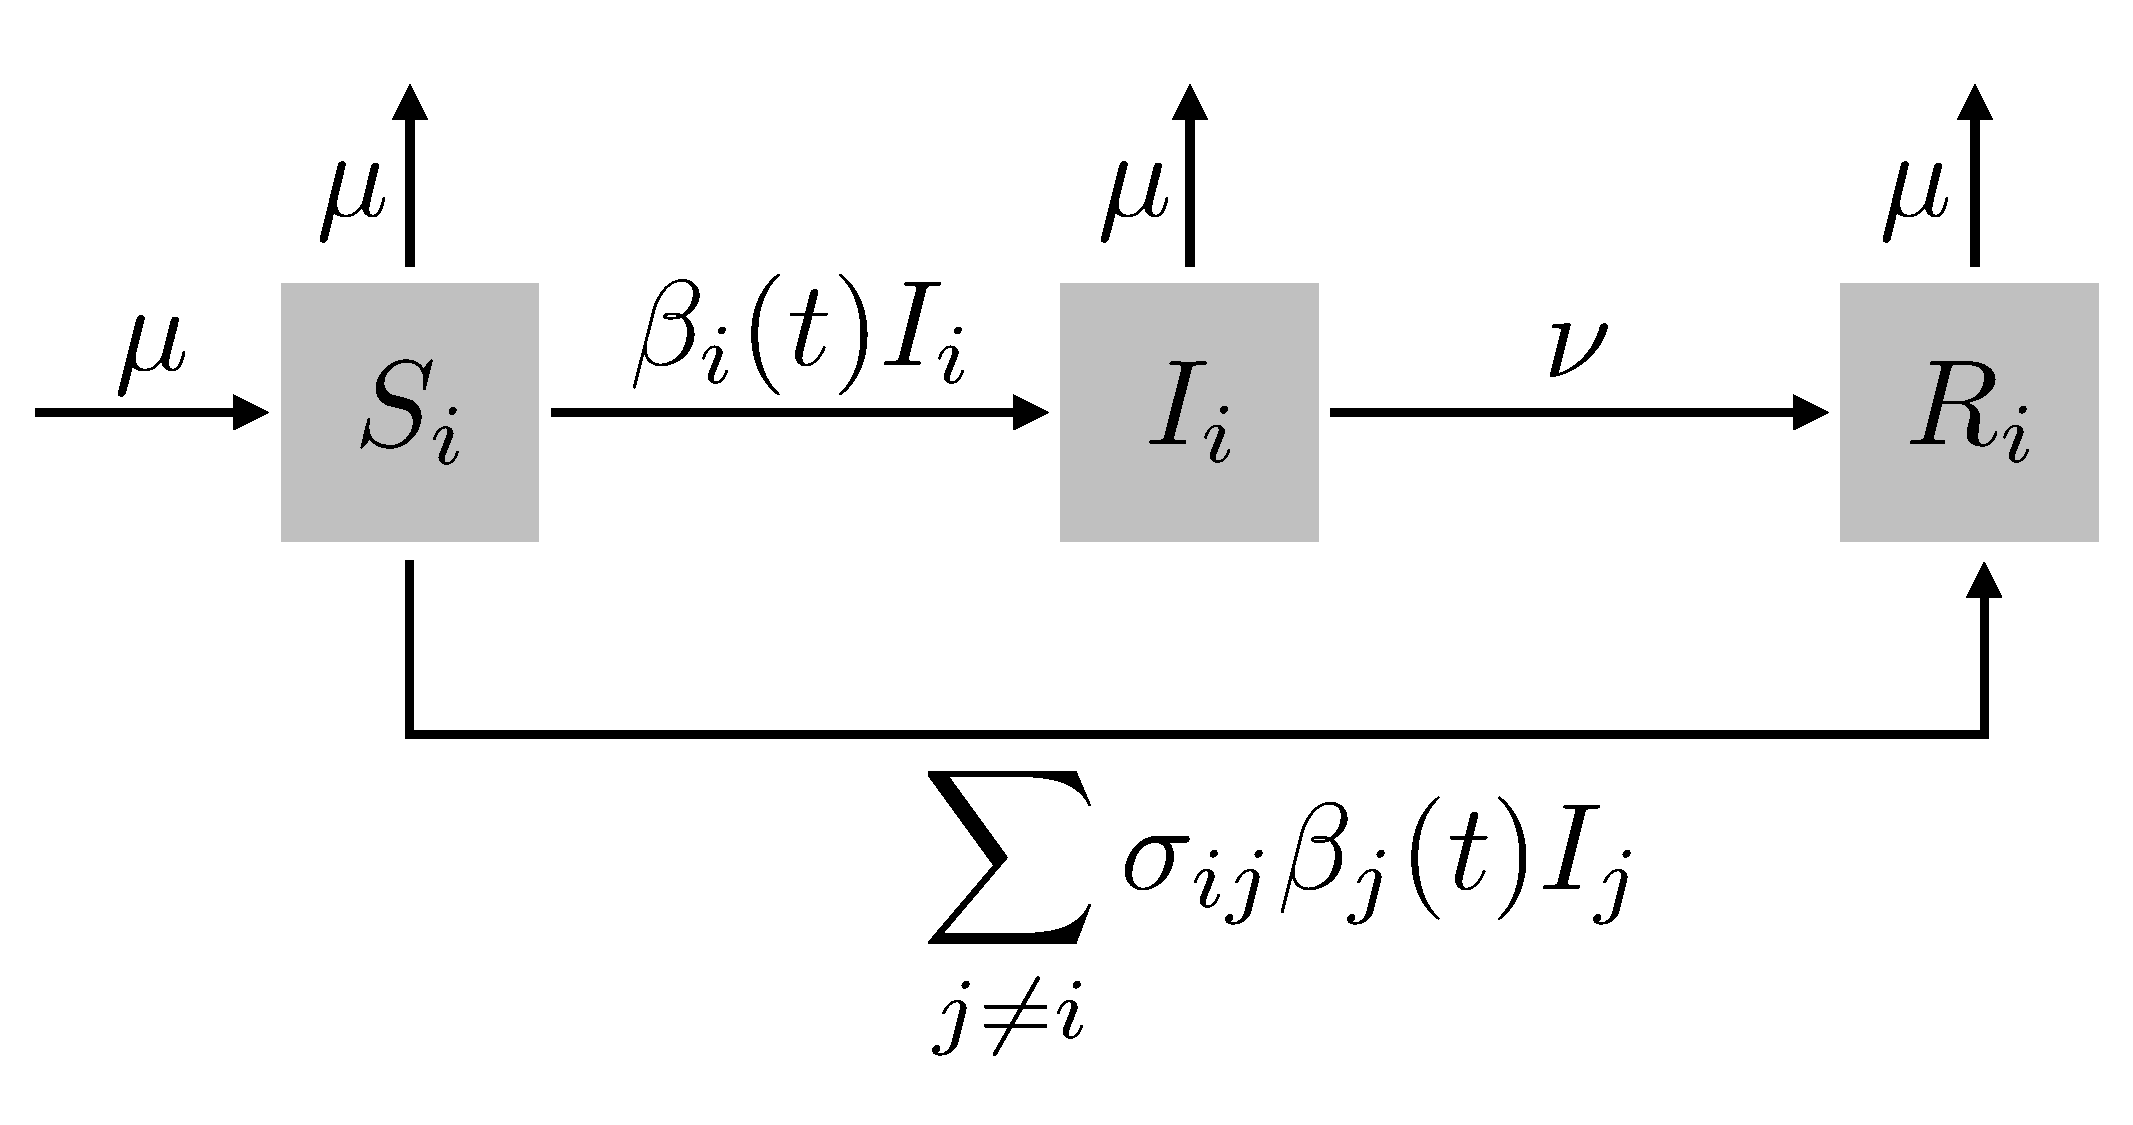
\includegraphics[width=5in]{dataflow/out/fig_compartmental/fig_compartmental.pdf}
    \end{center}
    \caption{\textbf{Compartmental representation of strain-competition model}.
    Hosts are susceptible (S), infected/infective (I), or recovered (R) with respect to each strain.
    Hosts move from S to I based on a seasonally varying transmission rate, and from I to R at a constant recovery rate. Competition takes place through cross-immunity, which is implemented by having hosts skip the infected state for one strain with some probability if they are already infected with another strain.
    \label{fig:compartmental}}
\end{figure}


Hosts enter the susceptible class for strain $i$ through the birth (and death) rate $\mu$. 
They leave through infection with strain $i$ ($S_i \to I_i$), infection with strain $j$ that elicits cross-immunity to $i$ ($S_i \to R_i$), or death.
The per capita transmission rate, $\beta_i(t)$, depends on a mean strain-specific rate, $\beta_i$, and a forcing function that is shared by all strains.
This function has a sinusoidal form and represents a shared common driver, such as seasonal changes in susceptibility or transmission from school-term forcing.
The forcing function is defined by a shared period $\psi$ and amplitude $\epsilon$.
Infected hosts recover at rate $\nu_i$ ($I_i \to R_i$).
The immune host class grows through these recoveries and also from the fraction of susceptible hosts, $S_i$, contacting infected hosts, $I_j$, who develop cross-immunity, $\sigma_{ij}$ ($0 \leq \sigma_{ij} \leq 1$).
Immunity of this form has been described as ``polarizing'' because $\sigma_{ij}$ of hosts $S_i$ contacting infecteds $I_j$ become completely immune (non-susceptible) to strain $i$, while $1-\sigma_{ij}$ remain completely susceptible.
This cross-immunity is a form of competition that determines the directions of interaction between strains: when $\sigma_{ij}>0$, strain $j$ drives strain $i$.
We assume $\sigma_{ii}=1$: hosts acquire perfect immunity to a strain from which they have recovered.

Process noise on the per capita transmission rate produces stochastic differential equations in Ito form:
\begin{align}
dS_i &=
	[\mu - \mu S_i] \, dt
	- S_i\sum\limits_{j} \sigma_{ij} \beta_j(t) I_j [dt +\eta \, dW_{t,j}] 
	\\
dI_i &= 
	\beta_i(t) S_i I_i [dt +  \eta \, dW_{t,i}]
	- [\nu_i + \mu] I_i \,  dt \\
dR_i &=
	[\nu_i I_i - \mu R_i] \, dt
	+ S_i\sum\limits_{j \neq i} \sigma_{ij} \beta_j(t) I_j [dt +  \eta \, dW_{t,j}]
\end{align}
where the $W_i$ are independent Wiener processes, one for each pathogen $i$, and $\eta$ represents the standard deviation of the noise as a fraction of the deterministic transmission rate.

The observations consist of the number of new cases or incidence over some interval. 
Cumulative cases $c_i$ at time $t$ were obtained by summing the $S_i \to I_i$ transitions from the start of the simulation through time $t$.
The incidence over times $t-\Delta t_\text{obs}$ to $t$, written as $C(t)$ for convenience, is given by the difference in cumulative cases:
\begin{align}
C_i(t) &= c_i(t_2) - c_i(t_1) \\
dc_i &= \beta_i(t) S_i I_i [dt + \eta \, dW_{t,i}]
\end{align}

\begin{table}
\caption{Default parameter values.}
\begin{center}
\begin{tabular}{cccc}
{\bf Symbol} &{\bf Description} & {\bf Default value} \\ 
\hline
$\beta_1, \beta_2$ & transmission rates & 0.3, 0.25 $\text{d}^{-1}$ \\
$\sigma_{12}$ & immunity to strain 1 from infection with 2 & see text\\
$\sigma_{21}$ & immunity to strain 2 from infection with 1 & 0\\
$\sigma_{ii}$ & homologous immunity for strain $i$ & 1\\
$\mu$ & birth and death rate & 1/30 $\text{y}^{-1}$ \\
$\nu$ & recovery rate & 0.2 $\text{d}^{-1}$ \\
$\epsilon$ & amplitude of seasonal forcing & 0.1 \\
$\psi$ & period of seasonal forcing & 360 d\\
$\eta$ & standard deviation of process noise & see text \\
$\text{S(0)}$ & initial fraction susceptible & see text \\
$\text{I(0)}$ & initial fraction infected & see text\\
$\Delta t_\text{obs}$ & incidence and sampling interval & 30 days\\
\end {tabular}
\end{center}

\label{table:defaultParameters}
\end{table}

\subsection*{Simulation}

The equations were solved numerically using the Euler-Maruyama method with a fixed step size. 
The step size was chosen to be less than the smallest within-run harmonic mean step size across deterministic, adaptive-step size pilot runs performed across the range of parameter space being studied. 
When numerical errors arose during transients, the step size was reduced further until the numerical issues disappeared.

Except where noted, the model was simulated with random initial conditions, and 1000 years of monthly observations were obtained from stochastic fluctuations around the deterministic attractor.
The use of random initial conditions minimizes arbitrary bias in the simulated dynamics.
From visual inspection of dynamics, the transient phase lasted much less than 1000 years. Time series were obtained from years 2000-3000.


\subsection*{Cross-mapping}

Convergent cross-mapping (CCM) is a method for inferring causality in deterministic systems via delay embedding~\cite{Sugihara2012}.
Takens' theorem holds that, for an $E$-dimensional system, the attractor for the state space represented by delay vectors in a single variable $X$, $\mathbf{x}(t) = \{X(t), X(t - \tau_1), X(t - \tau_2), \ldots , X(t - \tau_{E-1}) \}$, is topologically equivalent to the $E$-dimensional attractor for variables $X_1, ..., X_E$.
In the limit of infinite data, the full $E$-dimensional attractor can be reconstructed perfectly from a one-dimensional time series.
Therefore, because $\bx(t)$ contains complete information about the system's dynamics, if $Y$ is part of the same system and thus causally drives $X$, observations of $\bx(t) \rightarrow Y(t - \ell)$, for a fixed lag $\ell$, can be used to reconstruct unobserved values of $Y(t)$ from new observations of $\bx(t)$~(Fig.~\ref{fig:conceptual}).

To evaluate whether $Y$ drives $X$, we construct ``libraries'' of observations of $\bx(t) \rightarrow y(t - \ell)$.
For a particular library, we treat each value of $Y(t)$ as unobserved, and reconstruct its value $\hY(t)$ by identifying the $E + 1$ nearest neighbors to $\bx(t)$ in the library, $\bx(t_i)$, for $t_1, \ldots, t_{E+1}$, and calculating $\hY = \sum_{i = 1}^{E + 1} w_i Y(t_i)$.
In order to avoid predictability due to system autocorrelation rather than dynamical coupling, neighbors are restricted to be separated in time by at least three times the delay at which the autocorrelation drops below $1/e$.
Weights are calculated from the Euclidean distances $d_i$ between $\bx(t)$ and $\bx(t_i)$, with $w_i$ proportional to $\exp \left( -\frac{d_i}{d_0} \right)$, where $d_0$ is the distance to the nearest neighbor \cite{Sugihara2012}.

The cross-map correlation $\rho$ measures how well values of $Y$ can be reconstructed from values of $X$, and is defined as the Pearson correlation coefficient between reconstructed values $\hY(t)$ and actual values $Y(t)$ across the entire time series \cite{Ye2015}.
Given library size $L$ and lag $\ell$, we generate a distribution of cross-map correlations $\rho$ by bootstrap-sampling libraries mapping delay vectors $\bx(t)$ to values $Y(t - \ell)$ and then computing the cross-map correlation for each sampled library.
We use the bootstrap distribution of cross-map correlation as the basis for statistical criteria for causality.

\subsection*{Criteria for causality}

We infer causality using two primary criteria involving the cross-map correlation $\rho$ \cite{Sugihara2012, Ye2015}: (1) whether $\rho$ increases with $L$ for a fixed lag $\ell$, and (2) whether $\rho$ is positive and maximized at a negative temporal lag $\ell$. 
We also consider a weaker alternative to the first criterion, which is simply whether $\rho$ is positive.

\paragraph{Criterion 1}
If $Y$ drives $X$, then increasing the library size $L$ should improve predictions of $\bx(t)$ as measured by $\rho$~\cite{Sugihara2012} for fixed lag $\ell = 0$.
The first criterion tests for this increase in $\rho$ with $L$.
We calculate $\rho$ at $L_{\min} = E + 2$, the smallest library that will contain $E + 1$ nearest neighbors for delay vectors $\bx(t)$, and at $L_{\max}$, the total number of delay vectors $\bx(t)$ in the time series.
An increase in $\rho$ is indicated by a lack of overlap between the distributions at $L_{\min} = E + 2$, the smallest library that will have $E + 1$ neighbors for most points, and $L_{\max}$, the largest possible library given the time-series length and delay embedding parameters $E$ and $\tau$.

\paragraph{Criterion 2}
If $Y$ strongly drives $X$, cross-map correlation at $\ell = 0$ may yield a false positive when testing for $X$ driving $Y$, but because information is transferred forwards in time from $Y$ to $X$, the cross-map correlation should be maximized at a negative lag $\ell$~\cite{Ye2015}.
The second criterion simply requires that, to infer that $Y$ drives $X$, the cross-map correlation $\rho$ be maximized at a negative cross-map lag $\ell$ and be positive.
In other words, not only must $X$ contain information about $Y$, but this information must be greatest for past states of $Y$, reflecting the correct temporal direction for causality.


\subsection*{Statistical tests for causality criteria}

The theory underlying CCM assumes completely deterministic interactions and infinite data.
If $Y$ drives $X$ in the absence of noise, the correlation $\rho$ between the reconstructed and observed states of $Y$ should converge to one with infinite samples of $X$.
In practice, if $X$ and $Y$ share a complex (e.g., chaotic) attractor, time series of $X$ may not be long enough to see convergence~\cite{Sugihara2012}.

The presence of observation and/or process noise violates the deterministic assumptions and prevents $\rho$ from ever reaching 1.
Nonetheless, a detectable increase in the correlation $\rho$ with the library length $L$ (for Criterion 1), or a maximum and positive correlation at negative lag (for Criterion 2), may suffice to demonstrate that $X$ drives $Y$ in natural systems.
It is important to note that we have no formal theoretical justification for such statistical heuristics.

Our statistics are based on the distributions obtained from bootstrapping.
For Criterion 1, which tests for an increase in $\rho(L)$, we perform a nonparametric test of whether $\rho(L_{\max})$, obtained at the largest library length is greater than $\rho(L_{\min})$, obtained at the smallest libary length.
The p-value for this test is calculated as the probability that $\rho(L_{\max})$ is not greater than $\rho(L_{\min})$, and calculate the p-value directly from the sampled distributions (the fraction of bootstraps in which $\rho(L_{\max}) < \rho(L_{\min})$).
We also consider a weaker alternative, testing simply whether $\rho$ is significantly positive.

For Criterion 2, which tests whether the best cross-map lag is negative and thus indicates the correct causal direction in time, we perform a similar nonparametric test.
We identify the negative cross-map lag $\ell^{(-)}$ with the highest median correlation, $\rho(\ell^{(-)})$ as well as the nonnegative cross-map lag $\ell^{(0+)}$ with the highest median correlation.
The p-value for this test is calculated as the probability that $\rho(\ell^{(-)})$ is not greater than $\rho(\ell^{(0+)})$.

We use a significance threshold of $p<0.05$ for all tests.

\subsection*{Choice of delay and embedding dimension}
The theory underlying attractor reconstruction works with any $E$-dimensional projection of a one-dimensional time series, which can be generated in many ways from lags of the time series.
In simulated, deterministic models, $E$ can be known perfectly, but the best projection may be system-dependent.
In systems with process noise, unknown dynamics, and/or finite observations, there is no clearly superior method to select the appropriate projection \cite{Casdagli1991,Nichkawde2013,Uzal2011,Pecora2007, Cao1997, Small2004}.

We accommodated this uncertainty by using four different methods.
Two methods infer the best delay-embedding for each interaction by maximizing the ability of one variable, the driven variable, to predict itself (akin to nonlinear forecasting \cite{Sugihara1990, Sugihara1994}).
The third method instead uses the delay-embedding that maximizes the cross-mapping correlation $\rho$ for each interaction.
Three of the four methods use uniform embeddings, identifying $E$ and a fixed delay $\tau$, and the other uses a nonuniform embedding, identifying a series of specific delays $\tau_1$, $\tau_2$, etc., whose length determines $E$.

\begin{enumerate}
\item \textit{Univariate prediction method}: By default, for each causal interaction ($C_i \rightarrow C_j$), $E$ and $\tau$ are chosen to maximize the one-step-ahead univariate prediction $\rho$ at $L_{\max}$ for the driven variable ($C_j$) based on its own time series.
\item \textit{Maximum cross-correlation method}: As an alternative, $E$ and $\tau$ are chosen to maximize the mean cross-map correlation $\rho$ at $L_\text{max}$ for each causal interaction being tested, for each time series.
\item \textit{Random projection method}: A recently proposed method based on random projection of delay coordinates sidesteps the problem of choosing optimal delays \cite{Tajima2015}. Instead, for a given $E$, all delays up to a maximum delay $\tau_{\max}$ are projected onto an $E$-dimensional vector via multiplication by a random projection matrix. $E$ is chosen to maximize the cross-map correlation $\rho$.
\item \textit{Nonuniform method}: For each driven variable $C_j$, starting with $\tau_0 = 0$, additional delays $\tau_1, \tau_2, \ldots$ are chosen iteratively to maximize the directional derivative to nearest neighbors when the new delay is added \cite{Nichkawde2013}. The delays are bounded by the optimal uniform embedding based on a cost function that penalizes irrelevant information \cite{Uzal2011}. This method can be seen as a nonuniform extension of the method of false nearest neighbors \cite{Kennel1992}.
\end{enumerate}


\subsection*{Code}
Code implementing the state-space reconstruction methods is publicly available at \url{https://github.com/cobeylab/pyembedding}.
The complete code for the analysis and figures is publicly available at \url{https://github.com/cobeylab/causality_manuscript}; individual analyses include references to the Git commit version identifier in the `pyembedding' repository.
The simulated time series on which the analyses were performed are available from the authors on request.

\subsection*{Data on childhood infections}
Time series were obtained from L2-level data maintained by Project Tycho \cite{vanPanhuis2013}.
All available cases of measles, mumps, pertussis, polio, scarlet fever, and varicella were obtained from the first week of 1906 through the last week of 1953 for New York City and Chicago.
Pertussis data were terminated in the 26th week of 1948 to limit the influence of the recently introduced pertussis vaccine.
Incidence was calculated by dividing weekly cases by a spline fit to each city's population size, as reported by the U.S. Census.
